\documentclass[adobefonts, a4paper]{ctexart}

\usepackage[top=1.2in, bottom=1.2in, left=1in, right=1in]{geometry}
\usepackage{minted, graphicx, hyperref}

\hypersetup{colorlinks=true, linkcolor=blue}

\title{操作系统实验报告2}
\author{蔡日骏\quad12348003}

\begin{document}
\maketitle

\section{基本设计}
整个系统分为通用模块、引导程序、操作系统、用户程序四部分。下面分别介绍。

\subsection{通用模块}
由于BIOS中断调用使用比较麻烦,因此一些常用的功能,如屏幕输出、键盘输入、磁盘读取
等被封装到一个通用模块工具集\verb|utils|中。引导程序和操作系统编译后将要与这个模块
进行静态链接。但这个模块比较大,因此一些简单的用户程序并不需要链接到此模块。

\subsection{引导程序}
引导程序负责把操作系统加载到内存中,随后把控制权交给操作系统。为了模拟真实环境,
引导程序中人为加入了一些延迟。引导程序要求操作系统安装在第一个软盘驱动器的第一个
扇区开始的一段连续扇区内。操作系统占用的扇区数在引导程序编译时指定。引导程序将会
把操作系统加载到\verb|0x0500|开始的一段连续内存空间内。

\subsection{操作系统}
操作系统可用的内存为\verb|0x0500-0x7BFF|,大约有30KB的空间可用。操作系统带有简单
的控制台,能批量执行程序(单条命令连续执行多个操作,详见\nameref{usage})。由于文件
还没有做好,可用的用户程序的列表只能直接保存在分区表中,因此目前只支持4个用户程序,
用户程序名称不能超过13字节。

\subsection{用户程序}
从操作系统中启动的用户程序将被加载到\verb|0x07D0:0100|中,可用空间的线性地址为
\verb|0x7E00-0x7FFFF|,约480KB。用户程序使用纯二进制格式。此外,用户程序退出时
必须使用\verb|retf|指令返回操作系统。


\section{编译说明}
整个系统包含下面的源文件:

\begin{tabular}{|l|l|c|}
\hline
文件名&说明&格式\\ \hline
\verb|help.nasm|&用户程序,显示系统的帮助信息&nasm\\ \hline
\verb|loader.nasm|&引导程序&nasm\\ \hline
\verb|ls.nasm|&用户程序,列出可用的用户程序&nasm\\ \hline
\verb|Makefile|&Makefile&Makefile\\ \hline
\verb|os.nasm|&操作系统&nasm\\ \hline
\verb|program_list|&程序列表,记录用户程序的名称、位置、长度等&二进制\\ \hline
\verb|reboot.nasm|&用户程序,重新引导&nasm\\ \hline
\verb|stone.nasm|&用户程序,弹球&nasm\\ \hline
\verb|utils.nasm|&通用工具集模块&nasm\\ \hline
\end{tabular}

\vspace{\baselineskip}

编译时,运行如下命令即可,所有编译、链接、写入操作将会自动完成。
\begin{minted}{bash}
    $ make  # 编译引导程序和操作系统,生成可引导的软盘镜像
    $ make user_program  # 编译用户程序并安装到软盘镜像中
\end{minted}

编译需要有\verb|nasm|、\verb|ld|、\verb|dd|、\verb|make|。Makefile内容如下:

\begin{minted}{makefile}
LD=ld
LDFLAGS=
AS=nasm
ASFLAGS=

disk.img: os.bin loader.bin
    dd if=/dev/zero of=disk.img count=2880
    dd if=loader.bin of=disk.img conv=notrunc
    dd if=os.bin of=disk.img seek=1 conv=notrunc
    printf '\x55\xaa' | dd of=disk.img bs=1 seek=510 count=2 conv=notrunc

os.bin: os.o utils.o
    $(LD) $(LDFLAGS) -Ttext 0 --oformat binary -o $@ $^

loader.bin: loader.o utils.o
    $(LD) $(LDFLAGS) -Ttext 0 --oformat binary -o $@ $^

os.o: os.nasm
    # 64位Linux下生成ELF64格式目标文件,防止链接时出错
    $(AS) $(ASFLAGS) -f elf64 -o $@ $^d

loader.o: loader.nasm
    $(AS) $(ASFLAGS) -f elf64 -o $@ $^

utils.o: utils.nasm
    $(AS) $(ASFLAGS) -f elf64 -o $@ $^

user_programs: help.com ls.com reboot.com stone.com program_list disk.img
    dd if=help.com of=disk.img seek=3 conv=notrunc
    dd if=ls.com of=disk.img seek=4 conv=notrunc
    dd if=reboot.com of=disk.img seek=5 conv=notrunc
    dd if=stone.com of=disk.img seek=6 conv=notrunc
    dd if=program_list of=disk.img bs=1 seek=446 conv=notrunc

help.com: help.nasm
    $(AS) $(ASFLAGS) -o $@ $^

ls.com: ls.nasm
    $(AS) $(ASFLAGS) -o $@ $^

reboot.com: reboot.nasm
    $(AS) $(ASFLAGS) -o $@ $^

stone.com: stone.nasm
    $(AS) $(ASFLAGS) -o $@ $^

clean:
    -rm disk.img
    -rm -f *.o
    -rm -f *.bin
    -rm -f *.com
\end{minted}

\section{使用说明}\label{usage}
\subsection{简单命令}
在控制台中,输入\verb|?|命令可查看帮助;输入\verb|ls|命令可以列出所有已安装的用户程序;
输入\verb|reboot|命令可以重新引导系统;输入用户程序名称可执行指定的用户程序。上面列出
的三个命令同时也分别是三个用户程序。

\begin{center}
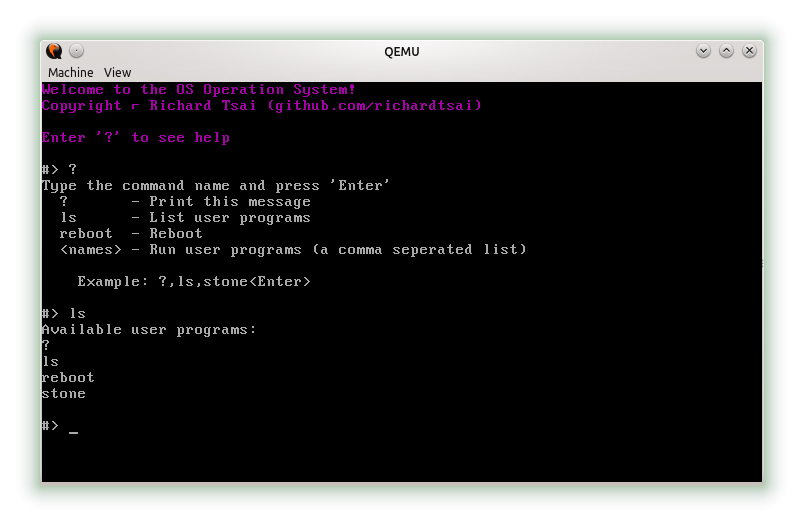
\includegraphics[scale=0.65]{single_cmd.png}
\end{center}

\subsection{批处理命令}
在控制台中,可以通过输入逗号分隔的多个简单命令来实现批处理。例如:

\begin{minted}{bash}
    #> ?,ls,stone
\end{minted}

可以按次序查看帮助信息、列出所有用户程序、运行\verb|stone|程序。

\begin{center}
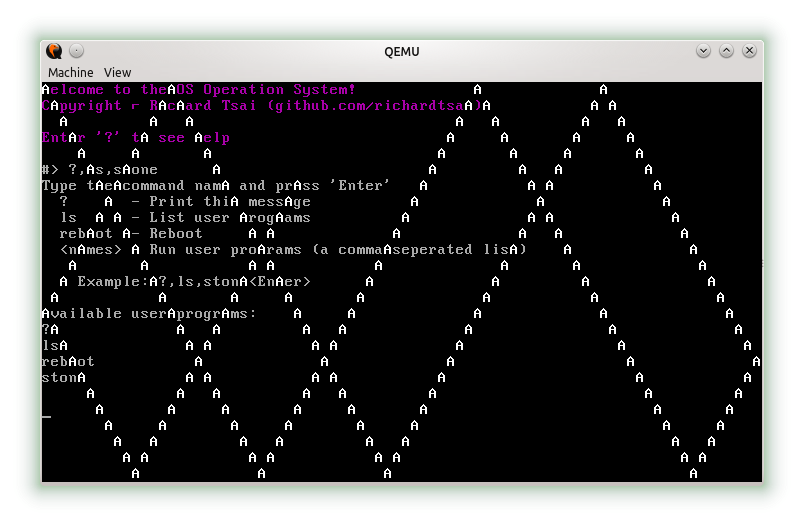
\includegraphics[scale=0.65]{multiple_cmd.png}
\end{center}

\end{document}
